
\section{Dataset Clustering Analysis}

We start with clustering all dataset with 11 features. Visual presentation of results above 3 dimension is not possible. Therefor we present the clustering results based on a pair of features in Fig.~\ref{fig:CxCy_11}. 

\begin{figure*}
    \centering
    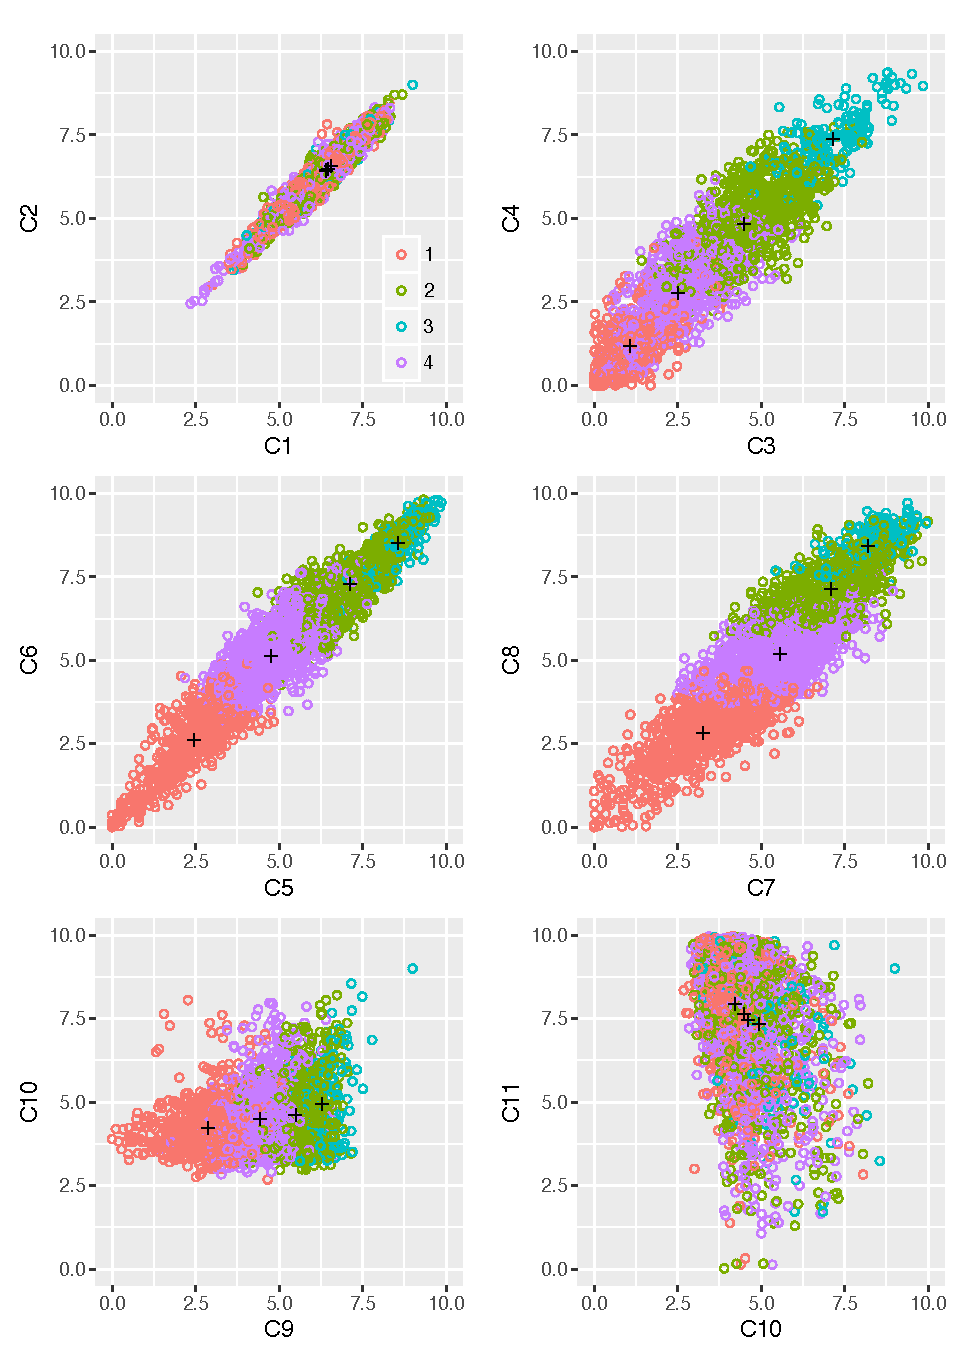
\includegraphics[width=\textwidth]{figures/pdf/Figure_5.pdf}
    \caption{Results of clustering analysis with all 11 attributes (metrics). This results are subsample of 55 possible combination of metrics. Center of cluster is shown as crosses. At this plot ordinal, categorical clusters' numbers are not necessarily represent the poor, fair, good, and excellent clusters. }
    \label{fig:CxCy_11}
\end{figure*}

The figure presents a part of results in clustering with 11 features. There are 55 other possibility to present (e.g., C1 vs C7 or C2 vs C9). As one can see in some combination of features the clustering patterns are easily seen. For example in C3 vs C4 we can distinguish 4 region for clusters, although they are partly mixed together. This also correct for C6 vs C7 and C7 vs C8. In the latter one we observe less mixture of data than the former one. Also there are other types of combination where one feature does not add so much information to the clustering process. For example in C9 vs C10, C10 could be considered as irrelevant feature. Irrelevant feature does not add further information for clustering and redundant feature add the equivalent information as the other feature \citep{Dy_2004_MLR}. The last combination of features are a good mixture of data and it is not possible to see the clustering boundaries. C1 vs C2 and C10 vs C11 are examples of such features combinations. It is worth to mention that at this point the cluster numbers are not consistent with ordinal categorical numbers of 1, 2, 3, and 4 representing poor, fair, good, and excellent, respectively.

Although we do not expect to see the pattern that resulted from clustering using 11 features in presentation of only two, however, different studies show that the higher dimension reduce the effect of similarity based on distance. \citet{Parsons_2004_ACM} presented an illustrative example to show the effect of dimension in reducing the importance of the distance. Effect of higher dimensions in clustering has been well studied and many different methods are proposed to reduce this effect in the final results. Among them we can name  feature selection before, during, and after clustering, hybrid methods that use combination of methods to select the best subset of feature. \citet{Dy_2004_MLR} addressed two issues involved in developing an automated feature subset selection algorithm for unlabeled data. They illustrated the irrelevant and redundant features and proposed methods for evaluating candidate features using two performance criteria.

Subspace analysis is another technique to address the challenges with higher dimensional data in clustering process. Subspace clustering is an extension of traditional clustering which looks for different pattern using subset of features.  \citet{Parsons_2004_ACM} provided a list of algorithm for conducting subspace clustering and also some potential applications for them. The most common factor among these algorithm is the process to find a group of best subspaces through optimization process. An n-dimensional dataset has $2^n$ subspaces where it could be very costly and time consuming to evaluate all of them.

As we discussed earlier, there is not standard measures for evaluating clusters in the clustering literature also there is no single clustering assignment explains every application \citep{Dy_2004_MLR,Jain_1988_Book,Hartigan_1985_JOC}. The clustering process is strongly dependent on the application. A good example of the concept is clustering a whale, an elephant, and a tuna fish \citep{Jain_1999,Watanabe_1985_Book}.  Whales and elephants should be in the same cluster, because they both are mammals. However, regarding the scope of the clustering the user could put tuna fish and whales in the same cluster because both groups live in water. In this study we are interested in using those features who, in general, represent the simulation accuracy in 4 different categories. As a first step we use the constrained \kmeans{} clustering approach for all features, however, because of mentioned reasons the results are not easy to discuss or even evaluate. Although we have four groups of data, the question is which one should be considered as poor, fair, good, or excellent groups. Therefore, we apply a modified method of subspace clustering approach to cluster the stations. As we discussed earlier and presented in figures the constrained \kmeans{} method effectively put the stations in a cluster with considering the fact that our constrain stations should not be in the same cluster. High number of iteration leads the clustering process to follow the clustering concept that we are looking for which is clustering stations as poor, fair, good, and excellent. In our case number of possible subspace is $2^{11}$ where each features have two options wether belong to subspace or not. However, because of preserving the distance based criteria effects we limited the number of features in the subspace to be 2,3, and 4 features. Therefor we have 330,165, and 55 unique subspaces for 4D,3D, and 2D, respectively. We conduct a constrained \kmeans{} clustering analysis for each of these subspaces and repeat the algorithm. In some cases, it is not possible to distinguish all four cannot-link stations in different clusters. In this study we ignore these cases. We only use those combination of features that gives 4 unique clusters for the constraint points (hypothetical stations), therefore, we know for sure that all data within same cluster let's say with metric value 3, should be considered as poor. We also control the clusters to be consistent (we reformat numbers to assign cluster 1 to all group of stations that our first constraint belongs to them and so on). Finally, using 550 unique subspace clustering results, we assign the most frequent class to the station. 

Fig.~\ref{fig:C_cvm_comp} shows the results for different velocity models and components after clustering the dataset. A preliminary visually inspection shows that the behavior of scores with respect to the velocity model is fairly similar. Therefor we merge data of different velocity models.  and present them at Fig.~\ref{fig:Figure_cluster_comp}. 

\begin{figure*}
    \centering
    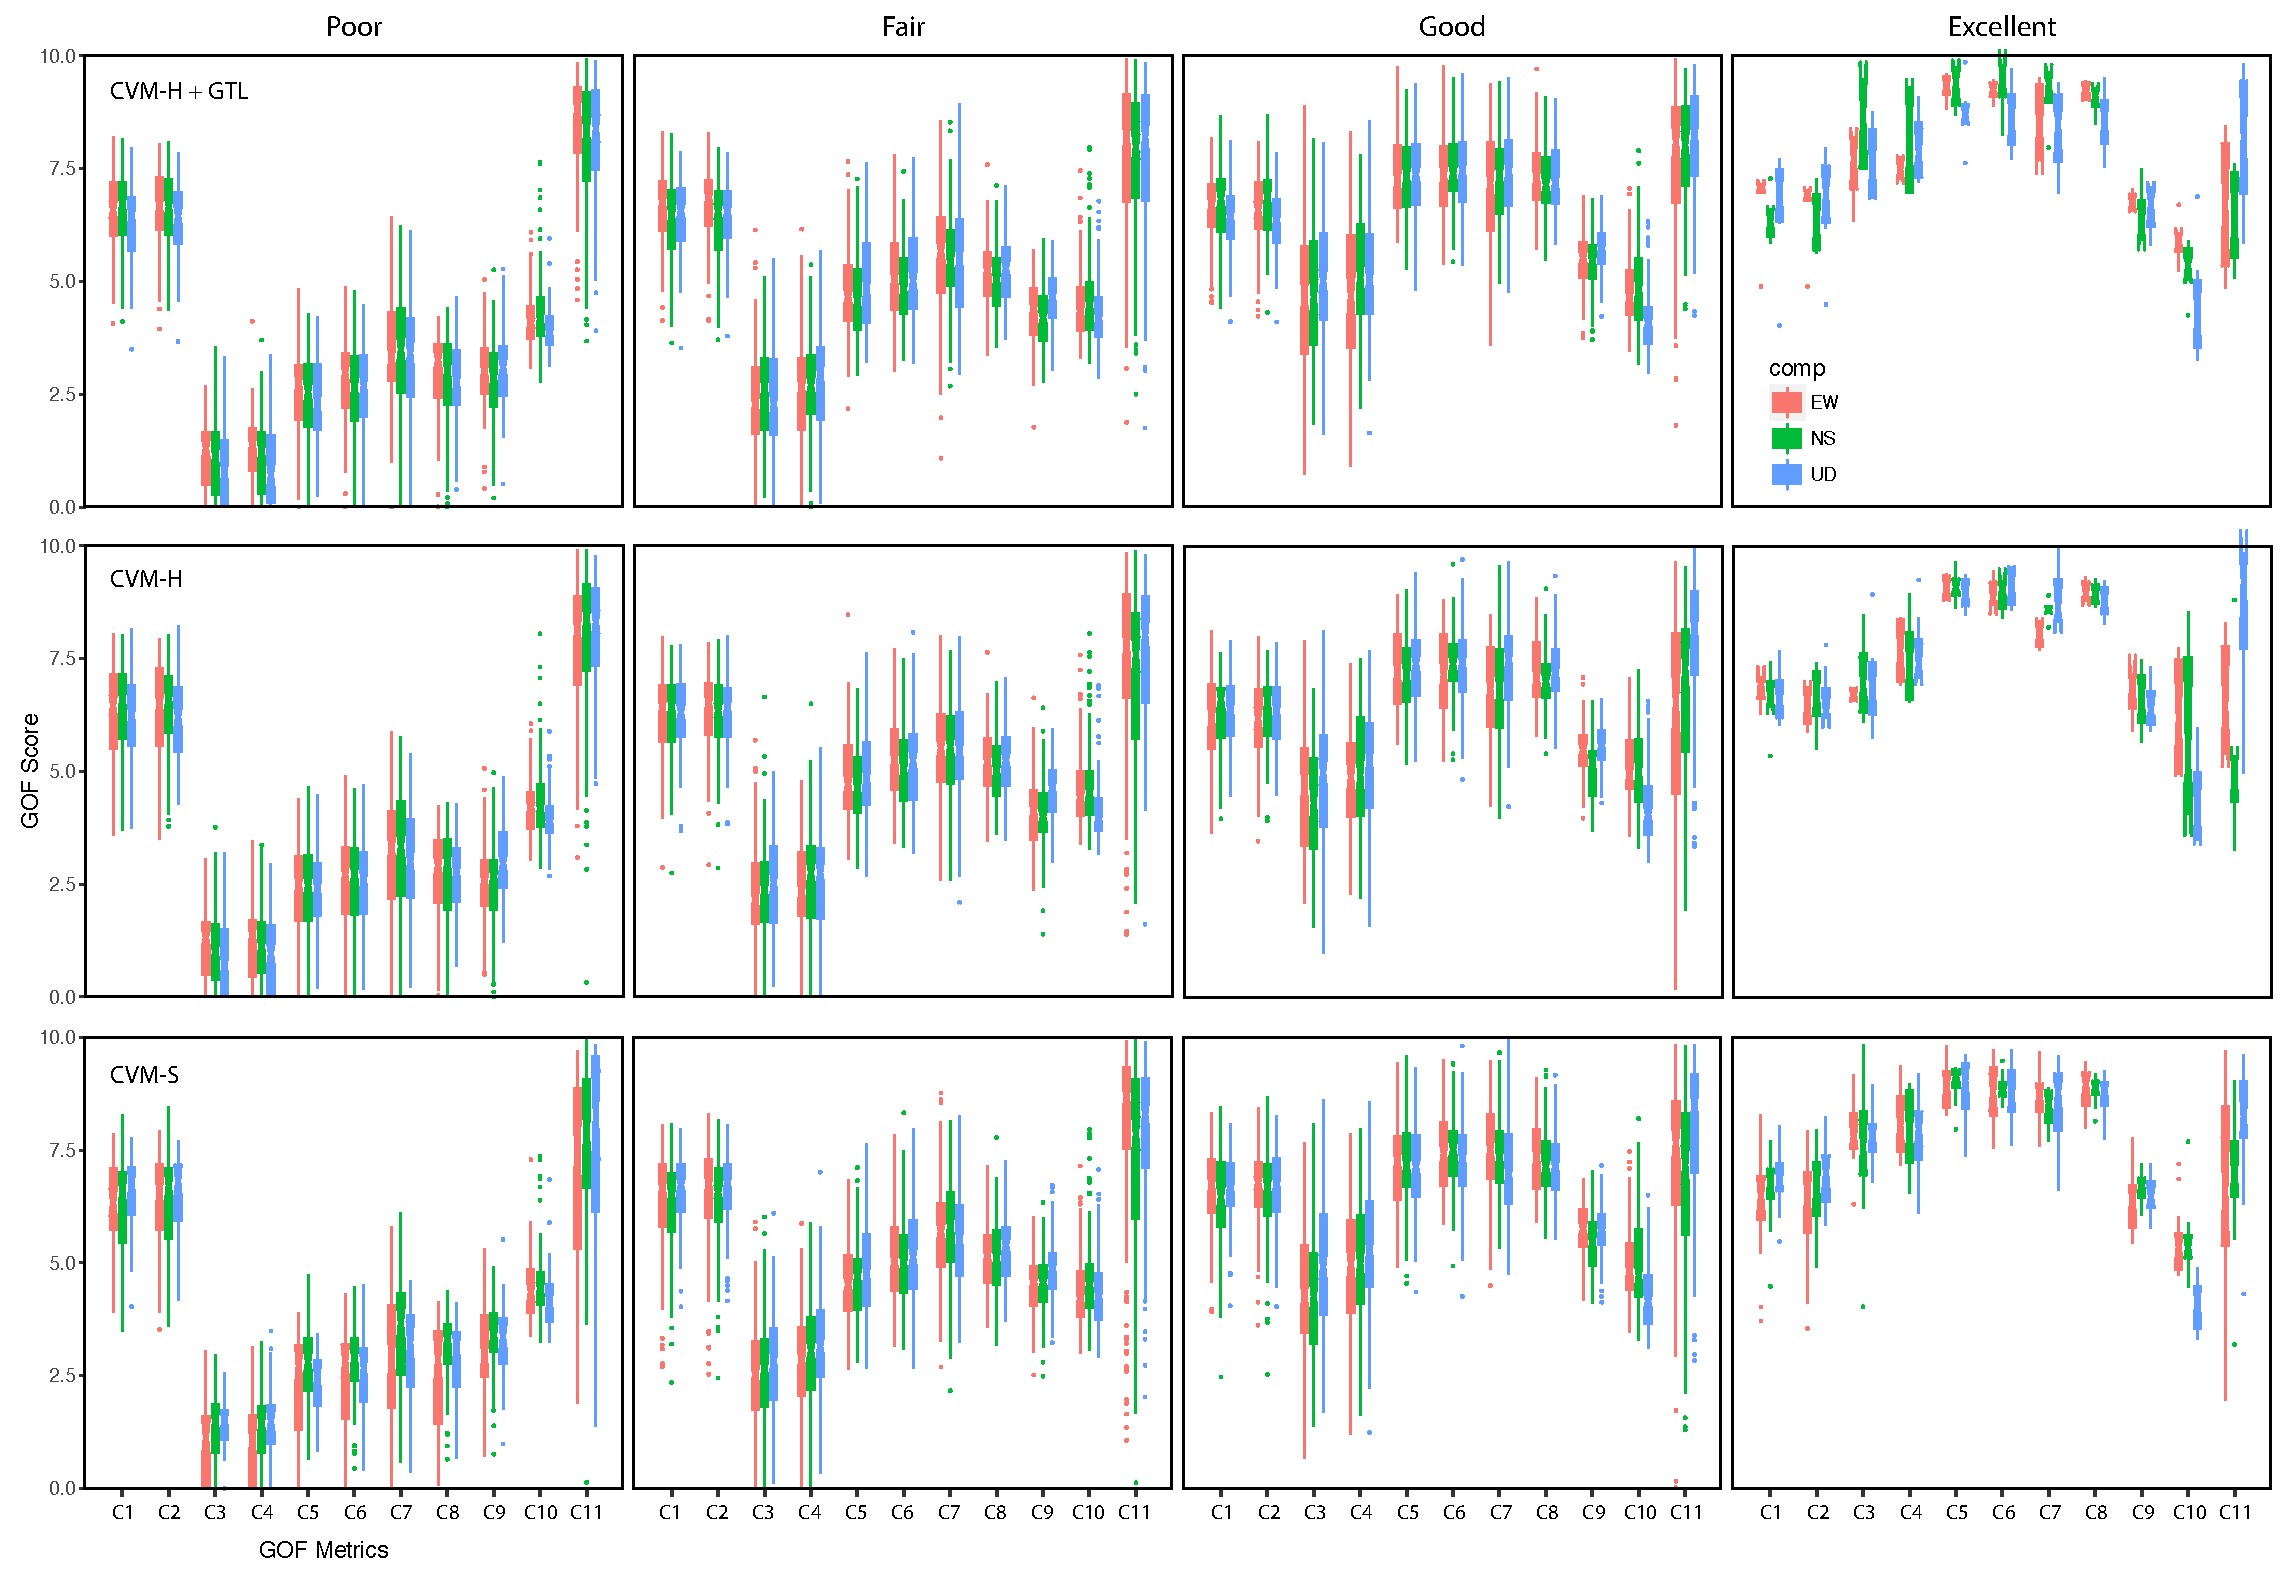
\includegraphics[width=\textwidth]{figures/pdf/Figure_6.pdf}
    \caption{Box plot of data used in the study after clustering. Metrics are shown for C1 to C11 for 3 components in separate plots for velocity models and clusters. Median of data are shown as notchs. Thick lines represent the IQR (Interquartile Range, Q3-Q1) of data. Outliers (data less than Q1-1.5*IQR and greater than Q3+1.5*IQR) are shown as scatter dots above and below plots if applicable.}
    \label{fig:C_cvm_comp}
\end{figure*}

\begin{figure*}
    \centering
    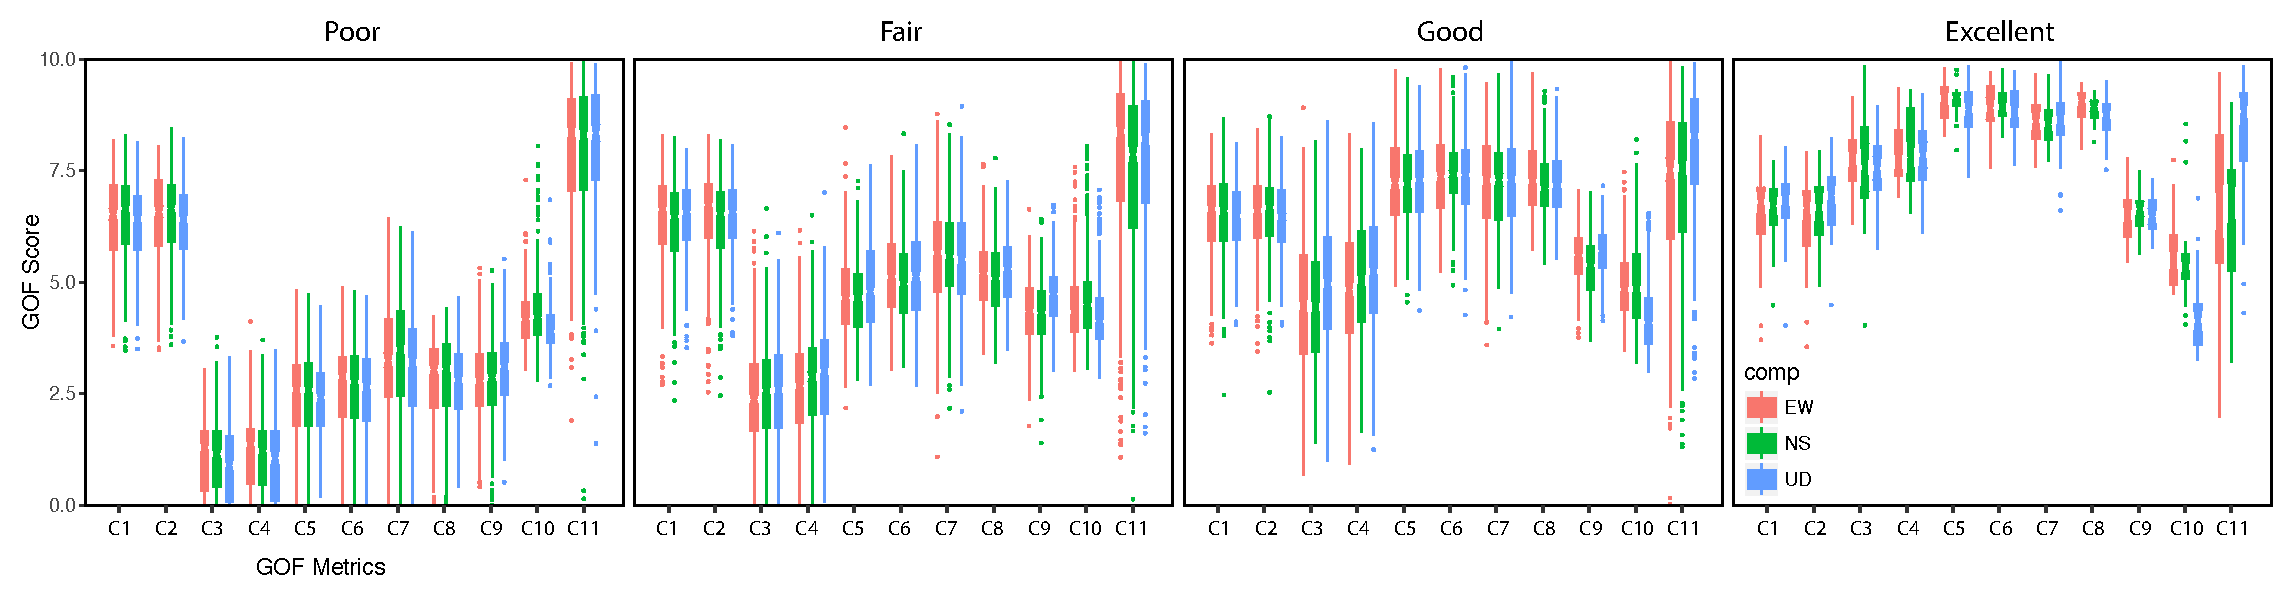
\includegraphics[width=\textwidth]{figures/pdf/Figure_7.pdf}
    \caption{Box plot of data used in the study after clustering and merging the results for different velocity models. Metrics shown for C1 to C11 for 3 components in separate plots for  clusters. Median of data are shown as notchs. Thick lines represent the IQR (Interquartile Range, Q3-Q1) of data. Outliers (data less than Q1-1.5*IQR and greater than Q3+1.5*IQR) are shown as scatter dots above and below plots if applicable.}
    \label{fig:Figure_cluster_comp}
\end{figure*}

Although there are some differences in the scores based on different components, there are general similarities in all clusters for different metrics among their components. Fig.~\ref{fig:Figure_cluster_all_comp} shows the results with merging the components. 

\begin{figure*}
    \centering
    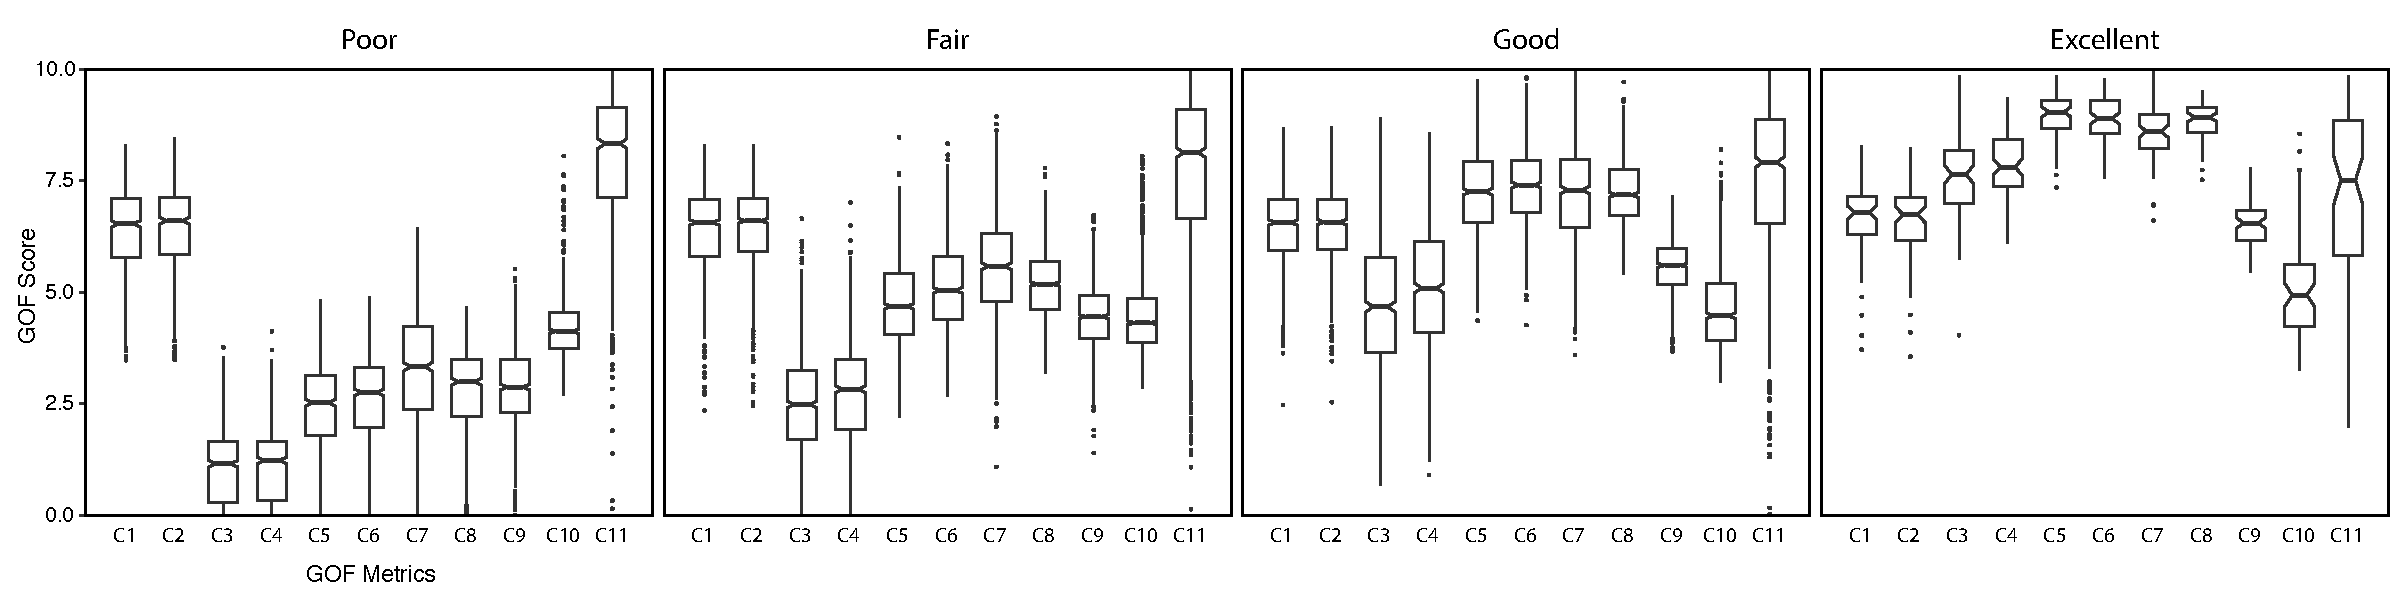
\includegraphics[width=\textwidth]{figures/pdf/Figure_8.pdf}
    \caption{Box plot of data used in the study after clustering and merging for different components and velocity models. Metrics shown for C1 to C11  in separate plots for  clusters. Median of data are shown as notchs. Thick lines represent the IQR (Interquartile Range, Q3-Q1) of data. Outliers (data less than Q1-1.5*IQR and greater than Q3+1.5*IQR) are shown as scatter dots above and below plots if applicable.}
    \label{fig:Figure_cluster_all_comp}
\end{figure*}

Fig.~\ref{fig:Figure_cluster_all_comp} presents the results from a broad perspective. Statistical tests can be helpful to understand the effect of component, velocity model, earthquake, and frequency band in the results.  According to Fig.~\ref{fig:Figure_cluster_all_comp} scores C1, C2, and C11 has the least changes in different clusters. It suggests the idea that they may not helpful in defining a decision rule. On the other hand, other scores are fairly variable among different clusters. 
Scores C1, C2, and C10 are very similar in cluster 1 to 3. However, we can see a small increase in cluster 4 for these scores. Also the data variation becomes small and range of data moves higher. Scores C3-C9 have a considerable increment from cluster 1 to cluster 4. Although there are a broad variation of data in cluster 3 and cluster 4 for these scores, good amount of data (50\% based on the IQR) are in a small range and increasing with respect to the clusters. C11 has a constant behavior with a small reduction in median at cluster 4. Fig.~\ref{fig:Figure_cluster_barplot} shows number of stations in each cluster based on component. 

\begin{figure}
    \centering
    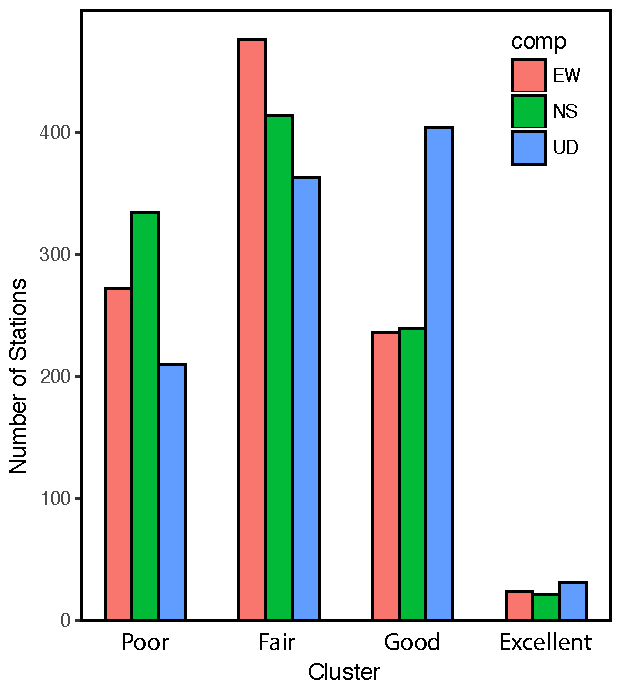
\includegraphics[width=\columnwidth]{figures/pdf/Figure_9.pdf}
    \caption{Number of data in each cluster based on components after conducting constraint \kmeans{} clustering through subspace analysis.}
    \label{fig:Figure_cluster_barplot}
\end{figure}



